% =====================================================================
% FJCAI 2027 -- paper skeleton.
%
% Built from FJCAI2027_Template_LaTeX.tex. ONLY the four marked blocks
% differ from the shipped template; everything else is byte-identical and
% must stay that way (the template says margins, columns, line spacing and
% fonts are prescribed).
%
% Compile with pdfLaTeX. XeLaTeX/LuaLaTeX WILL FAIL: \usepackage[utf8]{vietnam}
% is a pdfTeX-era package.
%
% Upload beside this file: IEEEtran.cls, fig1_architecture.pdf, fig2_pareto.pdf
% =====================================================================

\documentclass[9pt, conference, a4paper, compsocconf]{IEEEtran}
\usepackage{amsmath,amsxtra,amssymb,amsthm,latexsym,amscd,amsfonts}
\usepackage[utf8]{vietnam}
\usepackage[top=2.7cm, bottom = 5.4cm, left=2.72cm, right = 2.85cm]{geometry}
\headsep = 0.7cm
\headheight = 1.0cm
\footskip = 1.0cm
\voffset = -0.74 cm
%%%%
\usepackage{balance}

\usepackage{fancyhdr}
\pagestyle{fancy}
\usepackage{cite}
\usepackage{algorithmic}
\usepackage{graphicx}
\usepackage{textcomp}
\usepackage{booktabs}
\usepackage{tabularx}
\usepackage{xcolor}
\usepackage{amsmath,amsxtra,amssymb,amsthm,latexsym,amscd,amsfonts}
\usepackage{pgfplots}
\usepackage{multirow}
\usepackage{subcaption}
\pgfplotsset{compat=1.17}

\usepackage{tikz}
\usetikzlibrary{positioning}
\usetikzlibrary{arrows.meta}
\usetikzlibrary{shapes}
\usetikzlibrary{calc}
\usetikzlibrary{fit}
\usepackage[english]{babel}
\usepackage{fancyhdr}
\pagestyle{fancy}
\renewcommand{\sectionmark}[1]{\markright{\MakeUppercase{#1}}{}}
\renewcommand{\headrulewidth}{0pt}
\ifCLASSINFOpdf
\usepackage[pdftex]{graphicx}
  \DeclareGraphicsExtensions{.pdf,.jpeg,.png,.jpg}
\else
\usepackage[dvips]{graphicx}
  \DeclareGraphicsExtensions{.eps}
\fi
\usepackage{array}

\usepackage{caption}
\captionsetup{
  font={footnotesize},
  justification=centering,
  singlelinecheck=false
}
\usepackage[font=footnotesize]{subfig}

% ---------------------------------------------------------------------
% CHANGE 1 of 4: conference year 2026 -> 2027 (appears 3x in this file).
% CONFIRM the day/month and city with the organizers before submitting:
% the shipped template says "Cần Thơ, 27-28/3/2026" and only the YEAR is
% changed below. If FJCAI 2027 moves city or dates, edit those too.
% ---------------------------------------------------------------------
\makeatletter
\def\ps@IEEEtitlepagestyle{%
\def\@oddhead{\hfil \small{\textit{Hội thảo khoa học Quốc gia về Trí tuệ nhân tạo 2027 (FJCAI) - Cần Thơ, 27-28/3/2027}\hfil}%
	\def\@evenhead{\hfil\small{\textit{Hội thảo khoa học quốc gia về Trí tuệ nhân tạo 2027 (FJCAI) - Cần Thơ, 27-28/3/2027}\hfil}}%
		\def\@oddfoot{\scriptsize \thepage \hfil }%
		\def\@evenfoot{\scriptsize \hfil \thepage}
	}
}

\def\@maketitle{%
  \newpage
  \null
  \begin{center}%
    {%
      \fontsize{16}{18}\selectfont
      \bfseries \@title \par
    }%
    \vskip 4em%
    {%
    \fontsize{9}{3.5}\selectfont
      \begin{tabular}[t]{c}%
        \@author
      \end{tabular}\par
    }%
  \end{center}%
  \par
}

\renewenvironment{abstract}
  {\normalfont
   \@IEEEabskeysecsize
   \setlength{\parindent}{0pt}
   \noindent
   \if@twocolumn
     \bfseries\textit{\abstractname}:
   \else
     \begin{center}\textbf{\abstractname}\end{center}
   \fi}
  {\par}

\renewenvironment{IEEEkeywords}
  {\normalfont
   \@IEEEabskeysecsize
   \vspace{0.3em}
   \setlength{\parindent}{0pt}
   \noindent
   {\bfseries\itshape \IEEEkeywordsname: }\ignorespaces}
  {\par}

\def\IEEEbibitemsep{1.5pt plus .5pt}
\makeatother

% The shipped template sets these to "Tóm tắt" and "Từ khóa". The paper is in
% English, so both are overridden here. \abstractname must stay inside
% \AtBeginDocument: babel sets it at \begin{document} and would otherwise win.
\makeatletter
\AtBeginDocument{
  \renewcommand{\abstractname}{Abstract}
}
\renewcommand{\IEEEkeywordsname}{Index Terms}
\makeatother

\begin{document}
\pagenumbering{gobble}
\fontsize{9}{10}
\selectfont

\fancyhead[RE,LO]{\centering{\small{\textit{Hội thảo khoa học Quốc gia về Trí tuệ nhân tạo 2027 (FJCAI) - Cần Thơ, 27-28/3/2027}}}}

% ---------------------------------------------------------------------
% CHANGE 2 of 4: title and authors
% ---------------------------------------------------------------------
\title{Do Context Clusters Help Lightweight Image Classification?\\ An Ablation Study and a Stronger All-Local Baseline}

\author{\IEEEauthorblockN{Nguyen Viet Hung\IEEEauthorrefmark{1}, Nguyen Ba Nam\IEEEauthorrefmark{1}, Le Hoang Thai\IEEEauthorrefmark{1}}
	\IEEEauthorblockA{\IEEEauthorrefmark{1}Faculty of Information Technology, University of Science, VNU-HCM, Vietnam}
	\IEEEauthorblockA{Email: 23122032@student.hcmus.edu.vn, 23122043@student.hcmus.edu.vn, lhthai@fit.hcmus.edu.vn}
}

\maketitle

\begin{abstract}
% The template warns against special characters, symbols or math here, so this
% paragraph is deliberately plain text with no inline math.
Lightweight image classification at low input resolution is usually limited by
model size rather than by arithmetic throughput, which makes accuracy at a
fixed parameter budget the operative figure of merit. We ask whether the
Context Cluster token mixer, introduced for 5.3M-parameter models at 224 by
224, keeps its benefit in that regime, and answer with single-change ablations
under a matched training budget, three seeds per configuration and paired
significance tests. It does not. Holding the stem, fold partitioning and block
depth fixed and removing the local convolutional branch costs 0.74 points on
Tiny-ImageNet, whereas removing the clustering branch instead gains 1.03
points at 10 percent fewer parameters. A hand-designed sparse local filter is
likewise matched by a plain learned 3 by 3 convolution while using 2.50 times
less activation memory. Scaling the resulting all-local design to the
parameter budget of ShuffleNetV2-x1.5, widening its depthwise kernels to 7 by
7 and training it with logit distillation reaches 61.21 plus or minus 0.40
top-1 on Tiny-ImageNet, against 59.72 plus or minus 0.14 for ShuffleNetV2-x1.5
trained identically from the same teacher, and 58.76 plus or minus 0.06 for
the ResNet-18 teacher itself, using 4.16 times fewer parameters and 2.41 times
fewer operations than that teacher. On CIFAR-10 it leads ShuffleNetV2-x1.5 by
0.82 points and matches the teacher at 4.25 times fewer parameters. The gain
is conditional on distillation and costs 2.41 times the operations of the
parameter-matched baseline; we report measured memory and latency in both
eager and graph-captured execution, and show that operation counts mispredict
measured latency by more than fourfold.
\end{abstract}

\begin{IEEEkeywords}
\textbf{\textit{lightweight image classification; ablation study; context cluster; knowledge distillation; efficient architectures}}
\end{IEEEkeywords}

\IEEEpeerreviewmaketitle

% ---------------------------------------------------------------------
% CHANGE 3 of 4: six-section body
% ---------------------------------------------------------------------
% Sections I, II, III (Fig. 1 floats inside the Methodology section)
% =====================================================================
% Sections I, II, III.  \input{} from main.tex.
% =====================================================================

\section{Introduction}
\label{sec:intro}

A classifier deployed on a phone or a microcontroller is usually limited by
how much memory its weights occupy, not by how many multiplications the
processor can retire. Storage, over-the-air update size and the resident
footprint of a model all scale with its parameter count, which is why the
lightweight vision literature reports parameters first. That makes a specific
question the operative one: at a fixed parameter budget, which design extracts
the most accuracy? This paper answers it for low-resolution inputs by holding
parameters fixed, training every model under the same budget, and measuring
cost on real hardware instead of inferring it from operation counts.

Context Cluster \cite{coc} offers an unusual answer. Instead of attention or
convolution it mixes tokens by clustering them, and it reports competitive
accuracy at 5.3M parameters on $224\times224$ inputs. Its authors are explicit
that the goal is a new perspective on visual representation rather than state
of the art. What remains untested is whether the mechanism survives
compression: at one to three million parameters and $32\times32$ inputs, each
clustering stage sees few points, and the fold partitioning that keeps
clusters populated at high resolution has little left to partition. We treat
this as an open empirical question about operating regime, not as a criticism
of the original work.

To answer it we build a hybrid block in which each stage splits its channels
between a clustering branch and a local convolutional branch in ratio $\rho$,
and then vary one decision at a time: $\rho$, the fold partitioning, channel
shuffle, the stem stride, cluster occupancy, and the choice of local operator.
Every configuration trains for the same number of epochs on the same recipe,
repeats over three seeds, and is compared both with a Welch test on the seed
means and with an exact paired McNemar test on the $10{,}000$ test
predictions. Where a configuration has fewer than three seeds we say so in the
table.

The ablations point one way. Removing the local branch while holding the stem,
folds, depth and width fixed --- the comparison that isolates clustering from
everything it is usually bundled with --- costs $0.74$ pp. Removing the
clustering branch instead gains $1.03$ pp, at 10\% fewer parameters. Fold
partitioning and channel shuffle change accuracy by less than run-to-run
variation. The largest single effect in the whole study is the stem stride, at
$-5.72$ pp, and because stride~2 halves the resolution entering every
subsequent stage, most of that belongs to resolution rather than to anything
specific to clustering. At this scale the local branch carries the accuracy
and the clustering branch is a net cost.

Following that conclusion produces a design with no clustering in it at all.
Scaled to 2.71M parameters, given $7\times7$ depthwise kernels, and trained
with logit distillation, it reaches $61.21 \pm 0.40$ on Tiny-ImageNet. It
leads a parameter-matched ShuffleNetV2-x1.5 \cite{shufflenetv2} by $1.49$ pp
and its own ResNet-18 teacher by $2.46$ pp, both significant over seeds and
confirmed by a paired test on every seed individually. We chose
ShuffleNetV2-x1.5 as the primary baseline because an earlier version of our
model lost to it, and we report it rather than substituting something weaker.

Two caveats belong in the opening rather than buried later. The win holds
under distillation; with plain cross-entropy the margin over
ShuffleNetV2-x1.5 falls to $0.47$ pp and does not reach significance, and the
model merely ties its teacher. And the accuracy is bought with compute: at
matched parameters the proposed model performs $2.41\times$ the operations of
ShuffleNetV2-x1.5, though still $2.41\times$ fewer than the ResNet-18 it beats.

This paper contributes a controlled ablation of context clustering in the
lightweight low-resolution regime and the negative conclusion that it does not
pay for itself there; an all-local configuration that beats a
parameter-matched baseline and its own teacher on two datasets; a cost
protocol using graph-verified latency, per-batch-size memory reset and
weights reported separately from activations, together with the observation
that operation counts mispredict measured latency by more than fourfold; and
a release of every configuration, seed, per-image prediction and provenance
record behind the numbers.

% ---------------------------------------------------------------------
\section{Related Work}
\label{sec:related}

\textbf{Lightweight convolutional networks.} MobileNetV2 \cite{mobilenetv2}
established the inverted residual with a linear bottleneck, and ShuffleNetV2
\cite{shufflenetv2} argued that operation counts are a poor proxy for latency,
proposing four design rules derived from measured speed instead. Its channel
split, depthwise convolution and channel shuffle give a strong
accuracy-per-parameter trade-off, and the x1.5 width multiplier lands close to
the budget we study, which is why we adopt it as the primary baseline.
ConvNeXt \cite{convnext} later showed that widening depthwise kernels from
$3\times3$ to $7\times7$ buys roughly $0.7$ pp on ImageNet at negligible cost,
and RepLKNet \cite{replknet} pushed the idea further and attributed the gain
to effective receptive field rather than capacity. Our final design uses both
observations.

\textbf{Token mixers.} MetaFormer \cite{metaformer} separated the transformer
block into a token mixer and a channel MLP and showed that the surrounding
structure matters more than the mixer itself, which makes the mixer a clean
unit of ablation. Context Cluster \cite{coc} substitutes a clustering
operation: points are assigned to centres by similarity, aggregated, and
dispatched back. Reported results are at 5.3M parameters and $224\times224$.
We keep the MetaFormer skeleton fixed and vary only the mixer, which is what
lets a single number be attributed to clustering rather than to the
architecture around it.

\textbf{Knowledge distillation.} Hinton et al. \cite{hinton} match a student
to a teacher's softened logits, and the technique is routine in lightweight
vision because it closes part of the gap to a larger model at no inference
cost. Decoupled knowledge distillation \cite{dkd} separates the target and
non-target components of that loss and reweights them. A recurring difficulty
in comparisons is that distillation is often applied only to the proposed
model; we apply the identical recipe, teacher and seed to every student in
this paper, and report cross-entropy results alongside.

% ---------------------------------------------------------------------
\section{Methodology}
\label{sec:method}

\subsection{The hybrid block and its design space}

Every model in this study is built from the same four-stage MetaFormer
skeleton \cite{metaformer}. A block applies normalisation, a token mixer, a
LayerScale parameter and a stochastic-depth path, adds the residual, and
repeats the pattern with a channel MLP of ratio~3. Stages are separated by
stride-2 point reducers that halve resolution and widen the channel count.

The hybrid block parameterises the token mixer by a local ratio $\rho$. Given
$C$ input channels it routes $\rho C$ to a local convolutional branch and
$(1-\rho)C$ to a clustering branch, concatenates the two, and fuses them with
a $1\times1$ convolution; an optional channel shuffle precedes the split. The
clustering branch follows \cite{coc}: the feature map is divided into fold
tiles, centres are proposed within each tile, points are assigned to centres
by cosine similarity, aggregated, and dispatched back. Occupancy $r$, the
number of points per centre, is set by the proposal grid. Setting $\rho = 0$
recovers a pure clustering model and $\rho = 1$ removes clustering entirely,
which is what makes $\rho$ the variable the study turns on. Section~\ref{sec:ablation}
reports each of these knobs varied in isolation.

\begin{figure*}[!t]
\centering
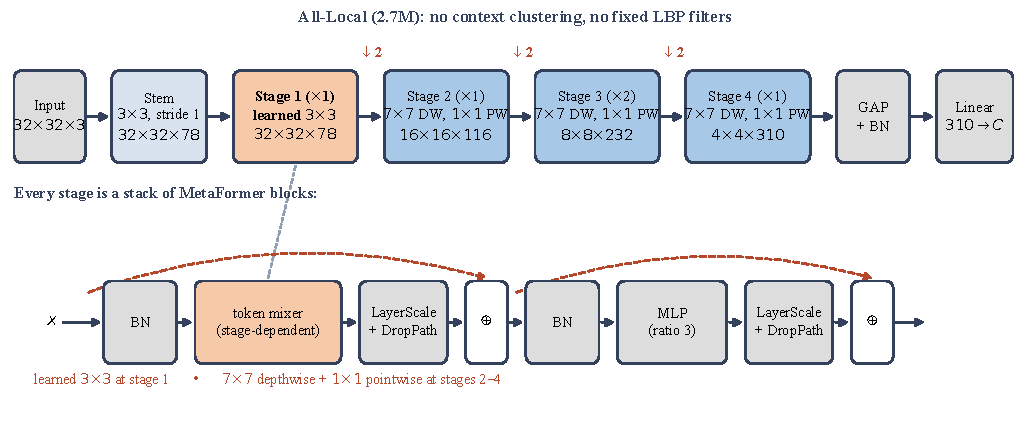
\includegraphics[width=\textwidth]{fig1_architecture.pdf}
\caption{The All-Local (2.7M) architecture. A stride-1 stem preserves the
$32\times32$ resolution into stage~1, whose token mixer is a learned
$3\times3$ convolution; stages~2--4 use $7\times7$ depthwise followed by
$1\times1$ pointwise convolution. Neither context clustering nor the fixed
LBP filters of the hybrid model appear in the final design.}
\label{fig:arch}
\end{figure*}

\subsection{The All-Local configuration}

The configuration the ablations select contains no clustering and no
hand-designed filters. Fig.~\ref{fig:arch} shows it.

The stem is a $3\times3$ convolution at stride~1, so stage~1 operates at the
full $32\times32$ resolution. This is the single most consequential choice in
the model: moving the stem to stride~2 costs $5.72$ pp
(Table~\ref{tab:ablation}), far more than any other decision we varied. At
$32\times32$ input there is little spatial information to discard, and
discarding half of it at the first layer is not recoverable downstream.

Stage~1 mixes tokens with a learned $3\times3$ convolution. The hybrid model
used fixed filters whose weights encode a sparse local binary pattern and
which expand the channel count eightfold before a pointwise projection;
Section~\ref{sec:ablation} shows that a plain learned convolution matches them
in accuracy at equal parameters while using $2.50\times$ less activation
memory, so we use the learned convolution.

Stages~2 to~4 mix tokens with a $7\times7$ depthwise convolution followed by a
$1\times1$ pointwise convolution. The wide kernel follows \cite{convnext}: with
only five blocks in the entire network, depth cannot grow the effective
receptive field, so each layer has to reach further, and a depthwise kernel
costs $k^2$ per channel rather than $C_\text{in}C_\text{out}k^2$. Widening
from $3\times3$ to $7\times7$ adds 35{,}600 parameters, 1.3\% of the model,
and 2.5M operations.

Channel widths are $[78, 116, 232, 310]$ with depths $[1, 1, 2, 1]$, giving
2{,}707{,}416 parameters with a 200-class head. The widths were chosen to
match ShuffleNetV2-x1.5 at 2{,}683{,}624 parameters so that the headline
comparison is at an equal budget; no other hyperparameter was tuned to the
baseline. A final normalisation, global average pooling and a linear
classifier complete the network.


\section{Experiments}
\label{sec:exp}
% =====================================================================
% Section IV: Experiments.  \input{} from main.tex inside \section{Experiments}.
% Every number here is traceable to a run in configs/run_plan.yaml; cost figures
% come from the single-session M1-v3 benchmark.
% =====================================================================

\subsection{Experimental Setup}
\label{sec:setup}

\textbf{Datasets.} We evaluate on Tiny-ImageNet \cite{tinyimagenet} (200
classes) and CIFAR-10 \cite{cifar} (10 classes). Both are processed at $32\times32$
resolution. For Tiny-ImageNet this means downsampling from the native
$64\times64$, which discards information and makes our absolute numbers
\emph{not} comparable to work that evaluates at $64\times64$; we adopt it
deliberately, because the regime this paper studies is low-resolution
classification under a tight parameter budget, and we hold it fixed across
every model so that all comparisons reported here are internally valid.
Tiny-ImageNet does not release labels for its test split, so we use the
official 10{,}000-image validation split as our \emph{test} set and hold out
a further 10{,}000 images from the training split, drawn with a fixed seed,
as the validation set used for model selection. No model ever selects an
epoch using the reported test set.

\textbf{Budget parity.} Every model, proposed or baseline, is trained for the
same number of epochs on a given dataset: 100 on Tiny-ImageNet and 250 on
CIFAR-10. We use identical augmentation --- RandAugment \cite{randaugment},
random erasing \cite{randomerasing}, mixup \cite{mixup} and CutMix
\cite{cutmix} --- the same optimiser and schedule, and the same batch size. No
model receives a tuned recipe of its own.

\textbf{Knowledge distillation.} Where distillation is used, every student,
\emph{including every baseline}, is distilled from a ResNet-18 teacher
\cite{resnet} trained on the same dataset and the same seed, with the same
loss: $\alpha = 0.5$ and temperature $T = 4$ \cite{hinton}. We report both
cross-entropy (CE) and distilled (KD) results for all models, so that no
comparison mixes training signals.

\textbf{Seeds and statistics.} Headline configurations are trained with three
seeds ($42, 43, 44$); tables report the mean and standard deviation, with the
number of runs $n$ given explicitly. Differences between groups are tested
two ways. At the seed level we use Welch's unequal-variance $t$-test on the
three per-seed accuracies. Within a seed we use an exact paired McNemar test
\cite{mcnemar} on the $10{,}000$ test predictions of the two models being
compared, which uses the pairing that a $t$-test over seed means discards. We report both
because they answer different questions, and we state $n$ wherever it is
below three.

\textbf{Counting operations.} Multiply--accumulate counts for the clustering
branch are easy to understate, and the first version of this work did. An
automatic counter sees the similarity matrix as a matrix product and counts
it, but the aggregation and dispatch steps are element-wise multiplications
followed by reductions, which most counters skip. For $N$ points, $M$ centres
per fold tile and head dimension $d$, each of the three steps costs $NMd$ per
head, so a counter that sees only the first reports a third of the branch's
arithmetic. We instrument the clustering operation directly and add the two
uncounted terms, which is why the operation counts we report for clustering
models are higher than a naive profile would give. For the proposed model the
correction is zero, since it contains no clustering.

\textbf{Reproducibility.} Every run writes a provenance record containing the
git commit, the seed, the resolved teacher checkpoint and the full software
and hardware environment, together with its per-image test predictions. The
code, the configuration of every run reported here, and those per-run records
are available at \url{https://github.com/nvhungus/context-cluster-ablation}.

% ---------------------------------------------------------------------
\subsection{Main Results}
\label{sec:main}

Table~\ref{tab:main} reports both datasets. Under distillation the proposed
All-Local model reaches $61.21 \pm 0.40$ top-1 on Tiny-ImageNet, against $59.72 \pm 0.14$ for
the parameter-matched ShuffleNetV2-x1.5 \cite{shufflenetv2} trained
identically from the same teacher. The margin of $+1.49$ pp is significant at
the seed level (Welch $t = 6.10$, $p = 0.016$) and, independently, on each of
the three seeds under a paired McNemar test. The same model exceeds the
ResNet-18 teacher that supervised it by $+2.46$ pp ($p = 0.008$) while using
$4.16\times$ fewer parameters and $2.41\times$ fewer multiply--accumulate
operations. The comparison holds on CIFAR-10, where
the proposed model leads ShuffleNetV2-x1.5 by $+0.82$ pp with distillation
(McNemar $p = 0.009$) and by $+0.64$ pp without it ($p = 0.014$), and is
statistically indistinguishable from the teacher ($-0.08$ pp validation,
$+0.15$ pp test, $p = 0.432$) at $4.25\times$ fewer parameters.

\textbf{The cross-entropy picture is weaker, and we state it plainly.}
Without distillation the proposed model reaches $58.69 \pm 0.10$ against
$58.22 \pm 0.23$ for ShuffleNetV2-x1.5. That $+0.47$ pp margin does not reach
significance at the seed level ($p = 0.051$), and against the ResNet-18
teacher the proposed model is $-0.07$ pp, a tie ($p = 0.405$). The
beat-the-teacher result reported above therefore holds \emph{in the distilled
setting}, and we condition every such claim on that setting rather than
presenting it as an unconditional property of the architecture.

\textbf{An asymmetry we observe but do not explain.} Given the identical
distillation recipe, the proposed model gains $+2.52$ pp from distillation
while ShuffleNetV2-x1.5 gains $+1.50$ pp and ShuffleNetV2-x1.0 gains $+1.58$
pp. The proposed design converts the same teacher signal into roughly one
additional percentage point. We note that this is not explained by headroom:
the proposed model has the \emph{higher} cross-entropy accuracy of the pair
and therefore less room to improve, yet gains more. We have not tested a
mechanism for this and do not propose one; we report it as an observation and
leave it to future work. What the comparison does establish is that under a
fixed, identical distillation protocol applied to every model, the proposed
architecture is the more accurate one at a matched parameter budget.

\textbf{A caveat about the MobileNetV2 row.} MobileNetV2 is the clear outlier
in Table~\ref{tab:main}: at 2.48M parameters it reaches $49.25$ on
Tiny-ImageNet, $6.53$ pp below a ShuffleNetV2-x1.0 that carries $41\%$ fewer
parameters. The cause is resolution, and part of it is our own adaptation.
Each of these networks was designed for $224\times224$ and reduces resolution
$32\times$ end to end, which leaves a $1\times1$ map at $32\times32$ input, so
all of them need their downsampling schedule shortened. For ResNet-18 and both
ShuffleNetV2 widths we removed two reduction steps, setting the stem to
stride~1 and replacing the max-pool with an identity, which leaves a
$4\times4$ final feature map. MobileNetV2 has no max-pool to remove, and we
changed only its stem stride; its four stride-2 inverted-residual stages
survive untouched, so it still reduces resolution $16\times$ and finishes on a
$2\times2$ map. Its operation count is the symptom: 25.8M MACs, the lowest in
the table and $1.8\times$ below ShuffleNetV2-x1.0 despite $70\%$ more
parameters. Most of its capacity sits in channels it can no longer resolve
spatially.

We report this because it means MobileNetV2 is a weaker baseline here than a
more carefully adapted version would be, and the weakness flatters our
results. It is also the reason we treat ShuffleNetV2-x1.5 rather than
MobileNetV2 as the primary comparison throughout. Read charitably, the row is
a second and independent instance of the effect that dominates
Section~\ref{sec:ablation}: at $32\times32$ the decisive variable is how early
a network discards spatial resolution, and a design that discards it twice
over cannot be rescued by parameters.

% Merged into one full-width float: the five-column single-column version
% overflowed \columnwidth and collided with the CIFAR-10 table. Keeping both
% datasets in one table* also removes the float-ordering hazard that arises
% when a table* and a table are queued separately.
\begin{table*}[!t]
\renewcommand{\arraystretch}{1.15}
\caption{\uppercase{Main results. Top-1 accuracy (\%) at $32\times32$, mean $\pm$ standard
deviation over $n$ seeds. Tiny-ImageNet: 100 epochs, $n$ as shown. CIFAR-10:
250 epochs, single seed. Every distilled student uses the same ResNet-18
teacher trained on the same dataset and seed, with $\alpha = 0.5$ and $T = 4$.
ResNet-18 is that teacher, so it is trained with cross-entropy only and has no
KD entry. Parameters and MACs are for the 200-class head; the CIFAR-10
variants differ only in the classifier.}}
\label{tab:main}
\centering
\footnotesize
\begin{tabular}{@{}lrrcccc@{}}
\toprule
& & & \multicolumn{2}{c}{Tiny-ImageNet} & \multicolumn{2}{c}{CIFAR-10} \\
\cmidrule(lr){4-5}\cmidrule(lr){6-7}
Model & Params & MACs & CE ($n$) & KD ($n$) & CE & KD \\
\midrule
ResNet-18 (teacher) \cite{resnet} & 11.27M & 556.8M & $58.76${\scriptsize$\pm$0.06} (3) & -- & $96.76$ & -- \\
MobileNetV2 \cite{mobilenetv2} & 2.48M & 25.8M & $49.25$ (1) & $52.32$ (1) & $94.06$ & $94.28$ \\
ShuffleNetV2-x1.0 \cite{shufflenetv2} & 1.46M & 46.3M & $55.78${\scriptsize$\pm$0.30} (3) & $57.36${\scriptsize$\pm$0.40} (3) & $95.40$ & $95.22$ \\
ShuffleNetV2-x1.5 \cite{shufflenetv2} & 2.68M & 96.1M & $58.22${\scriptsize$\pm$0.23} (3) & $59.72${\scriptsize$\pm$0.14} (3) & $95.56$ & $95.86$ \\
Context Cluster \cite{coc} & 2.46M & 34.4M & $49.45$ (1) & -- & $92.74$ & -- \\
Hybrid baseline ($\rho{=}0.5$) & 1.80M & 138.9M & $56.40${\scriptsize$\pm$0.21} (3) & $58.19${\scriptsize$\pm$0.25} (3) & $95.44$ & $96.16$ \\
\midrule
\textbf{All-Local (ours)} & 2.71M & 231.3M & $\mathbf{58.69}${\scriptsize$\pm$0.10} (3) & $\mathbf{61.21}${\scriptsize$\pm$0.40} (3) & $\mathbf{96.20}$ & $\mathbf{96.68}$ \\
\bottomrule
\end{tabular}
\end{table*}

% ---------------------------------------------------------------------
\subsection{Ablation Study}
\label{sec:ablation}

Table~\ref{tab:ablation} varies one design decision at a time from the hybrid
model, holding the stem, fold partitioning, block depth and width fixed so
that each row isolates a single factor.

\textbf{Clustering does not pay for itself.} Setting $\rho = 0$, which removes
the local convolutional branch and leaves pure clustering while keeping every
other choice identical, costs $0.74$ pp. Setting $\rho = 1$ instead, removing
the clustering branch entirely, \emph{gains} $+1.03$ pp while using 10\% fewer
parameters. The two rows bracket the question the paper asks: at this scale and
resolution the local branch is what carries the accuracy, and the clustering
branch is a net cost.

\textbf{The supporting design choices contribute little.} Removing fold
partitioning ($+0.20$ pp) and removing channel shuffle ($+0.25$ pp) both leave
accuracy unchanged within run-to-run variation, so neither is load-bearing.
Changing cluster occupancy in either direction hurts, by $1.02$ pp at $r = 1$
and $0.80$ pp at $r = 4$, and giving stage~4 four centres instead of one costs
$0.31$ pp. The single largest effect in the table is the stem stride: moving
from stride~1 to stride~2 costs $5.72$ pp. Because that change halves the
resolution entering every stage as well as altering cluster occupancy, we
attribute the bulk of it to resolution rather than to clustering.

\textbf{The hand-designed local operator is replaceable.}
Table~\ref{tab:operator} compares the fixed sparse LBP-pattern filters used at
stage~1 of the hybrid model against a plain learned $3\times3$ convolution at
matched parameters. At 1.62M parameters the learned convolution is ahead by
$0.10$ pp (McNemar $p = 0.63$); at the 2.71M scale of the proposed model the
two are indistinguishable over three seeds ($61.21 \pm 0.40$ against
$61.23 \pm 0.28$, Welch $p = 0.956$). The learned convolution nevertheless
uses $2.50\times$ less peak activation memory at batch 128, because the fixed
filters expand the channel count eightfold before projecting back. We
therefore adopt the learned convolution: the hand-designed operator buys no
accuracy and costs memory.

\begin{table}[!t]
\renewcommand{\arraystretch}{1.15}
\caption{\uppercase{One-change ablations on Tiny-ImageNet, cross-entropy.
Each row changes exactly one design decision from the hybrid baseline.}}
\label{tab:ablation}
\centering
\footnotesize
\begin{tabular}{@{}lccr@{}}
\toprule
Configuration & Top-1 (\%) & $n$ & $\Delta$ \\
\midrule
Hybrid baseline ($\rho{=}0.5$) & $56.40${\scriptsize$\pm$0.21} & 3 & -- \\
\midrule
$\rho = 0$ (clustering only) & $55.66${\scriptsize$\pm$0.20} & 3 & $-0.74$ \\
$\rho = 1$ (local only, 1.62M) & $57.43${\scriptsize$\pm$0.14} & 3 & $\mathbf{+1.03}$ \\
\midrule
No fold partitioning & $56.60$ & 1 & $+0.20$ \\
No channel shuffle & $56.65$ & 1 & $+0.25$ \\
Stage-4 $2\times2$ proposals & $56.09$ & 1 & $-0.31$ \\
Occupancy $r = 1$ & $55.38$ & 1 & $-1.02$ \\
Occupancy $r = 4$ & $55.60$ & 1 & $-0.80$ \\
Stem stride $1 \rightarrow 2$ & $50.68$ & 1 & $\mathbf{-5.72}$ \\
\bottomrule
\end{tabular}
\end{table}

\begin{table}[!t]
\renewcommand{\arraystretch}{1.15}
\caption{\uppercase{Stage-1 operator: fixed LBP-pattern filters against a learned
$3\times3$ convolution, at matched parameters. Memory is peak activation
memory at batch 128, in MB.}}
\label{tab:operator}
\centering
\footnotesize
\begin{tabular}{@{}llcrr@{}}
\toprule
Scale & Stage-1 operator & $n$ & Top-1 (\%) & Mem. \\
\midrule
\multirow{2}{*}{1.62M, CE} & fixed LBP & 1 & $57.31$ & 797 \\
 & learned $3\times3$ & 1 & $57.41$ & 317 \\
\midrule
\multirow{2}{*}{2.71M, KD} & fixed LBP & 3 & $61.23${\scriptsize$\pm$0.28} & 1037 \\
 & \textbf{learned} $\mathbf{3\times3}$ & 3 & $61.21${\scriptsize$\pm$0.40} & \textbf{415} \\
\bottomrule
\end{tabular}
\end{table}

% ---------------------------------------------------------------------
\subsection{Cost Analysis}
\label{sec:cost}

All cost figures in Table~\ref{tab:cost} are measured on a single NVIDIA
Tesla T4 (fp32, $32\times32$ input, 200-class head). Every model was profiled
in one session on the same host, so cross-model differences are not
confounded by hardware; we verified that re-profiling the same models in a
separate session leaves parameters, operation counts and peak memory
bit-identical but shifts batch-128 latency by up to 14\%, and we therefore
report a single session throughout. Latency is given both in eager execution
and with the forward pass captured in a CUDA Graph; every captured graph was
verified to reproduce its eager output bitwise, and each figure is the median
of five timed loops of 100 iterations after a warm-up of at least one second.
Peak memory is reset per batch size, and resident weights are reported
separately from activations.

At batch size one, the deployment-relevant operating point, the proposed model
occupies 10.37\,MB of weights and 22.58\,MB of peak memory, against 43.03\,MB
and 58.75\,MB for the ResNet-18 teacher: a $4.15\times$ reduction in model
size and a $2.60\times$ reduction in peak memory, together with $2.41\times$
fewer operations and a $2.18\times$ lower graph-captured latency (0.804\,ms
against 1.752\,ms), while being 2.46\,pp more accurate. Against the
parameter-matched ShuffleNetV2-x1.5 the proposed model uses $2.41\times$ more
operations, but the measured deployment cost is close: 22.58\,MB against
20.85\,MB of peak memory at batch one ($1.08\times$) and 0.804\,ms against
0.752\,ms of graph-captured latency ($1.07\times$). In eager execution the
ordering reverses and the proposed model is $1.72\times$ faster (3.50\,ms
against 6.03\,ms), because 87.5\% of ShuffleNetV2-x1.5's eager batch-one
latency is CPU kernel-launch overhead against 77.1\% for ours, a consequence
of its per-block channel split, shuffle and concatenation. At batch 128 the
proposed model remains the more expensive of the two, using 415.0\,MB against
133.0\,MB and reaching 3803 against 5768 images per second; we report this
because it is a regime our claims do not cover.

Two measurements caution against treating operation counts as a latency proxy.
First, realized arithmetic throughput at batch 128 varies by nearly tenfold
across the models evaluated: ResNet-18 performs $2.41\times$ more
operations than the proposed model yet completes a batch of 128 in 28.06\,ms
against 32.76\,ms, because dense $3\times3$ convolutions map onto far
better-optimised kernels than the bandwidth-bound depthwise--pointwise stacks
used by lightweight designs. Second, the relative ordering of two models can
invert between execution modes, as the ShuffleNetV2-x1.5 comparison above
shows. We therefore report both modes and draw deployment conclusions only
where they agree. Fig.~\ref{fig:pareto} places every model on the accuracy
against parameters and accuracy against operations planes; the proposed model
is on the Pareto frontier of the first and is not Pareto-dominant on the
second, and we claim only the former.

\begin{table*}[!t]
\renewcommand{\arraystretch}{1.15}
\caption{\uppercase{Measured cost on one NVIDIA Tesla T4, fp32, $32\times32$ input,
200-class head, all models profiled in a single session. Memory is peak
allocated; latency is the median of five timed loops.}}
\label{tab:cost}
\centering
\footnotesize
\begin{tabular}{@{}lrrrrrrrr@{}}
\toprule
& & & \multicolumn{2}{c}{Peak memory (MB)} & \multicolumn{3}{c}{Latency (ms)} & Throughput \\
\cmidrule(lr){4-5}\cmidrule(lr){6-8}
Model & Params & MACs & $b{=}1$ & $b{=}128$ & eager $b{=}1$ & graph $b{=}1$ & graph $b{=}128$ & (img/s) \\
\midrule
ResNet-18 (teacher) & 11.27M & 556.8M & 58.75 & 326.7 & 2.64 & 1.752 & 28.06 & 4709 \\
MobileNetV2 & 2.48M & 25.8M & 19.62 & 124.3 & 4.74 & 0.674 & 12.85 & 9970 \\
ShuffleNetV2-x1.0 & 1.46M & 46.3M & 15.72 & 95.6 & 6.07 & 0.680 & 13.44 & 9683 \\
ShuffleNetV2-x1.5 & 2.68M & 96.1M & 20.85 & 133.0 & 6.03 & 0.752 & 22.03 & 5768 \\
Hybrid baseline ($\rho{=}0.5$) & 1.80M & 138.9M & 19.70 & 481.6 & 7.68 & 1.212 & 36.47 & 3408 \\
\midrule
\textbf{All-Local (ours)} & 2.71M & 231.3M & 22.58 & 415.0 & 3.50 & 0.804 & 32.76 & 3803 \\
\bottomrule
\end{tabular}
\end{table*}

\begin{figure*}[!t]
\centering
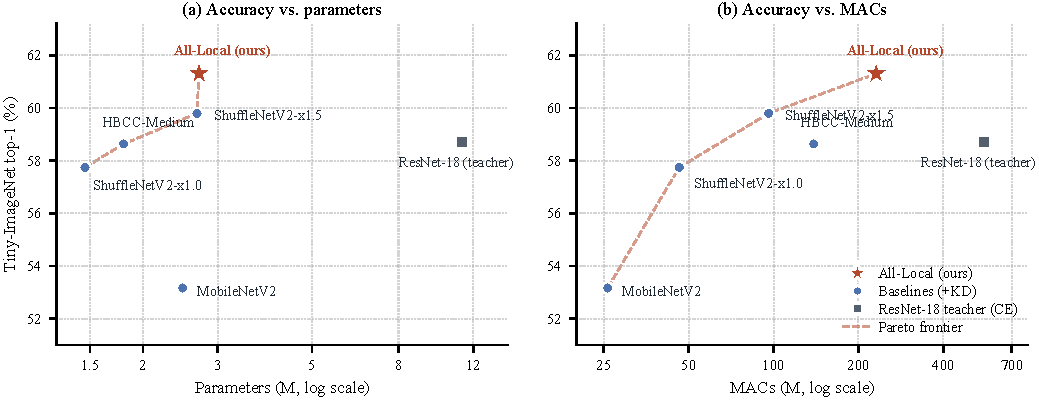
\includegraphics[width=\textwidth]{fig2_pareto.pdf}
\caption{Tiny-ImageNet accuracy against parameters (a) and against
multiply--accumulate operations (b), both on logarithmic axes. Accuracy is
the mean over three seeds; cost is measured on a Tesla T4 in a single
session. Every baseline shown is distilled from the same ResNet-18 teacher;
the teacher itself is trained with cross-entropy and is marked separately.
The proposed model lies on the parameter frontier but not on the operation
frontier.}
\label{fig:pareto}
\end{figure*}


% Sections V and VI
% =====================================================================
% Sections V and VI.  \input{} from main.tex.
% =====================================================================

\section{Discussion and Limitations}
\label{sec:limits}

The result we are most confident in is negative. Context clustering, inserted
into a fixed MetaFormer skeleton and compared against a convolutional branch
at the same parameter count, loses by $1.03$ pp at one to three million
parameters and $32\times32$ input. The supporting machinery built around it
--- fold partitioning, channel shuffle, a tuned occupancy --- moves accuracy
by less than seed variance, and the one setting that matters a great deal,
the stem stride, matters because of resolution rather than because of
clustering. None of this contradicts \cite{coc}, which reports a different
operating point; it bounds where the mechanism is useful.

The positive result is narrower than the headline number suggests, in three
specific ways.

\textbf{It depends on distillation.} Under cross-entropy the proposed model
leads ShuffleNetV2-x1.5 by $0.47$ pp, which does not reach significance over
three seeds ($p = 0.051$), and it does not beat the ResNet-18 teacher at all
($-0.07$ pp, $p = 0.405$). Only with distillation does the margin reach $1.49$
pp and the teacher comparison reverse. Every claim in this paper about
exceeding the teacher is therefore a claim about the distilled setting.

\textbf{We cannot explain the distillation asymmetry.} Given an identical
teacher, temperature and loss weight, the proposed model gains $2.52$ pp from
distillation while ShuffleNetV2-x1.5 gains $1.50$ pp and ShuffleNetV2-x1.0
gains $1.58$ pp. The obvious explanation, that a weaker model has more room to
improve, predicts the opposite of what we observe: the proposed model has the
higher cross-entropy accuracy and still gains more. We report the asymmetry
because it is what produces the headline margin, and we decline to attribute
a mechanism to it without a test. Establishing whether this is a property of
the architecture, of the width, or of the $7\times7$ kernels would need a
study of its own.

\textbf{The accuracy is paid for in compute.} At matched parameters the
proposed model performs $2.41\times$ the operations of ShuffleNetV2-x1.5,
occupies $3.12\times$ its peak memory at batch 128, and reaches $0.66\times$
its throughput. It is cheaper than the teacher it beats on every static axis
--- $4.16\times$ fewer parameters, $2.41\times$ fewer operations, $2.60\times$
less memory at batch one --- but against the parameter-matched baseline the
exchange is accuracy for compute, and a deployment limited by arithmetic
rather than by model size should prefer the baseline.

Two further limits constrain how far the numbers travel. Both datasets are
evaluated at $32\times32$, which for Tiny-ImageNet means downsampling from the
native $64\times64$; our absolute accuracies are therefore not comparable to
published results at the native resolution, and we make no such comparison.
And while every Tiny-ImageNet configuration is run with three seeds, the
CIFAR-10 results come from a single seed each; their significance rests on
paired tests over $10{,}000$ test images within that seed, which is a weaker
guarantee than seed-level replication.

% ---------------------------------------------------------------------
\section{Conclusion}
\label{sec:conclusion}

We set out to test whether context clustering earns its place in a lightweight
classifier at low resolution, and found that it does not: at a matched
parameter budget, replacing the clustering branch with a convolutional one
improves Tiny-ImageNet accuracy by $1.03$ pp while using fewer parameters, and
the design choices that surround clustering contribute less than seed
variance. Carrying that conclusion through yields a clustering-free model
which, at 2.71M parameters with $7\times7$ depthwise kernels and logit
distillation, reaches $61.21 \pm 0.40$ on Tiny-ImageNet and $96.68$ on
CIFAR-10, exceeding a parameter-matched ShuffleNetV2-x1.5 by $1.49$ pp and its
own ResNet-18 teacher by $2.46$ pp while using $4.16\times$ fewer parameters
than that teacher. The gain is conditional on distillation and costs
$2.41\times$ the operations of the parameter-matched baseline, and we report
both alongside the measured memory and latency rather than parameter counts
alone. The ablations, configurations, seeds and per-image predictions behind
every number are released.


\section*{Acknowledgement}
The authors would like to thank...

% ---------------------------------------------------------------------
% CHANGE 4 of 4: references. {99} reserves label width for 2-digit numbers.
% ---------------------------------------------------------------------
\balance
\begin{thebibliography}{99}

\bibitem{coc} X. Ma, Y. Zhou, H. Wang, C. Qin, B. Sun, C. Liu and Y. Fu,
``Image as set of points,'' in \emph{Proc. Int. Conf. Learning
Representations (ICLR)}, 2023.

\bibitem{metaformer} W. Yu, M. Luo, P. Zhou, C. Si, Y. Zhou, X. Wang,
J. Feng and S. Yan, ``MetaFormer is actually what you need for vision,''
in \emph{Proc. IEEE/CVF Conf. Computer Vision and Pattern Recognition
(CVPR)}, 2022, pp. 10819--10829.

\bibitem{hinton} G. Hinton, O. Vinyals and J. Dean, ``Distilling the
knowledge in a neural network,'' in \emph{NIPS Deep Learning and
Representation Learning Workshop}, 2015.

\bibitem{shufflenetv2} N. Ma, X. Zhang, H.-T. Zheng and J. Sun,
``ShuffleNet V2: Practical guidelines for efficient CNN architecture
design,'' in \emph{Proc. European Conf. Computer Vision (ECCV)}, 2018,
pp. 116--131.

\bibitem{mobilenetv2} M. Sandler, A. Howard, M. Zhu, A. Zhmoginov and
L.-C. Chen, ``MobileNetV2: Inverted residuals and linear bottlenecks,''
in \emph{Proc. CVPR}, 2018, pp. 4510--4520.

\bibitem{convnext} Z. Liu, H. Mao, C.-Y. Wu, C. Feichtenhofer, T. Darrell
and S. Xie, ``A ConvNet for the 2020s,'' in \emph{Proc. CVPR}, 2022,
pp. 11976--11986.

\bibitem{replknet} X. Ding, X. Zhang, J. Han and G. Ding, ``Scaling up your
kernels to 31x31: Revisiting large kernel design in CNNs,'' in
\emph{Proc. CVPR}, 2022, pp. 11963--11975.

\bibitem{resnet} K. He, X. Zhang, S. Ren and J. Sun, ``Deep residual
learning for image recognition,'' in \emph{Proc. CVPR}, 2016, pp. 770--778.

\bibitem{dkd} B. Zhao, Q. Cui, R. Song, Y. Qiu and J. Liang, ``Decoupled
knowledge distillation,'' in \emph{Proc. CVPR}, 2022, pp. 11953--11962.

\bibitem{tinyimagenet} Y. Le and X. Yang, ``Tiny ImageNet visual
recognition challenge,'' Stanford CS231N Technical Report, 2015.

\bibitem{mcnemar} T. G. Dietterich, ``Approximate statistical tests for
comparing supervised classification learning algorithms,''
\emph{Neural Computation}, vol. 10, no. 7, pp. 1895--1923, 1998.

% TODO: add the remaining references (target ~28 total).

\end{thebibliography}

\end{document}
